% =====================================================================
%  MẪU BÁO CÁO CHO SINH VIÊN - Nguyễn Tuấn Anh
%  Biên dịch bằng XeLaTeX (hoặc LuaLaTeX). Trên Overleaf: Menu > Compiler > XeLaTeX
% =====================================================================
\documentclass[12pt,a4paper,oneside]{report}

% Cỡ chữ thân bài 13pt (giống bản Word)
\makeatletter
\renewcommand\normalsize{%
  \@setfontsize\normalsize{13pt}{15.6pt}%
  \abovedisplayskip 12pt plus3pt minus7pt
  \belowdisplayskip \abovedisplayskip
  \abovedisplayshortskip 0pt plus3pt
  \belowdisplayshortskip 6.5pt plus3.5pt minus3pt}
\normalsize
\makeatother

% ---------------- Trang giấy & phông chữ ----------------
\usepackage[a4paper,left=2cm,right=2cm,top=2cm,bottom=3cm]{geometry}
\usepackage{fontspec}
\setmainfont{Times New Roman}
\usepackage[vietnamese]{babel}
\usepackage{setspace}
\setstretch{1.3}
\setlength{\parindent}{1cm}
\setlength{\parskip}{6pt}
\usepackage{indentfirst}

% ---------------- Gói hỗ trợ ----------------
\usepackage{graphicx}
\graphicspath{{images/}}
\usepackage{float}
\usepackage{array}
\usepackage{caption}
\captionsetup{labelsep=colon,font=normalsize,skip=6pt}
\usepackage{titlesec}
\usepackage{titletoc}
\usepackage{enumitem}
\usepackage{cite}          % gộp trích dẫn: [4-6], [2, 4-6]
\usepackage{fancyhdr}
\usepackage[hidelinks,unicode]{hyperref}

% ---------------- Đánh số trang (chân trang, giữa) ----------------
\pagestyle{fancy}
\fancyhf{}
\fancyfoot[C]{\thepage}
\renewcommand{\headrulewidth}{0pt}
\fancypagestyle{plain}{\fancyhf{}\fancyfoot[C]{\thepage}\renewcommand{\headrulewidth}{0pt}}

% ---------------- Tên gọi tiếng Việt ----------------
\addto\captionsvietnamese{%
  \renewcommand{\contentsname}{MỤC LỤC}%
  \renewcommand{\listfigurename}{DANH MỤC HÌNH ẢNH}%
  \renewcommand{\listtablename}{DANH MỤC BẢNG}%
  \renewcommand{\bibname}{TÀI LIỆU THAM KHẢO}%
  \renewcommand{\figurename}{Hình}%
  \renewcommand{\tablename}{Bảng}%
  \renewcommand{\chaptername}{Chương}%
}

% Hình đánh số theo chương (Hình 1.1), bảng đánh số liên tục (Bảng 1)
\renewcommand{\thefigure}{\thechapter.\arabic{figure}}
\counterwithout{table}{chapter}

% ---------------- Định dạng tiêu đề ----------------
% Chương: "Chương 1. Tổng quan về học máy" - 14pt, đậm, căn giữa
\titleformat{\chapter}[block]
  {\centering\bfseries\fontsize{14}{18}\selectfont}
  {\chaptername~\thechapter.}{0.5em}{}
\titlespacing*{\chapter}{0pt}{0pt}{18pt}
% Mục cấp 2: "1.1. Giới thiệu" - 14pt, đậm
\titleformat{\section}
  {\bfseries\fontsize{14}{18}\selectfont}{\thesection.}{0.5em}{}
\titlespacing*{\section}{0pt}{12pt}{6pt}
% Mục cấp 3: "1.4.1. Mục 1" - 13pt, đậm
\titleformat{\subsection}
  {\bfseries\fontsize{13}{17}\selectfont}{\thesubsection.}{0.5em}{}
\titlespacing*{\subsection}{0pt}{10pt}{6pt}

% Mục lục: ghi "Chương 1." trước tên chương
\titlecontents{chapter}[0pt]{\addvspace{4pt}\bfseries}
  {\chaptername~\thecontentslabel.\enspace}{}{\titlerule*[0.6pc]{.}\contentspage}
\titlecontents{section}[1.5em]{}
  {\thecontentslabel.\enspace}{}{\titlerule*[0.6pc]{.}\contentspage}
\titlecontents{subsection}[3em]{}
  {\thecontentslabel.\enspace}{}{\titlerule*[0.6pc]{.}\contentspage}

% Chương không đánh số (Mở đầu, Tài liệu tham khảo) vẫn có trong mục lục
\newcommand{\unnumberedchapter}[1]{%
  \chapter*{#1}\addcontentsline{toc}{chapter}{#1}}

% Bảng trống 3 cột làm mẫu
\newcolumntype{C}{>{\centering\arraybackslash}p{0.3\textwidth}}

\begin{document}

% =====================================================================
%  MỤC LỤC, DANH MỤC HÌNH, DANH MỤC BẢNG
% =====================================================================
\pagenumbering{arabic}
\tableofcontents
\clearpage
\phantomsection\addcontentsline{toc}{chapter}{DANH MỤC HÌNH ẢNH}
\listoffigures
\clearpage
\phantomsection\addcontentsline{toc}{chapter}{DANH MỤC BẢNG}
\listoftables
\clearpage

% =====================================================================
%  MỞ ĐẦU
% =====================================================================
\unnumberedchapter{Mở đầu}

Trong một báo cáo khoa học, báo cáo môn học hay báo cáo nghiên cứu, phần
Lời mở đầu (hoặc Mở đầu) thường được viết ngắn gọn, súc tích và cần đảm
bảo các nội dung sau:

\textbf{1. Giới thiệu bối cảnh và lý do chọn đề tài}

Nêu tình hình thực tiễn, lý do tại sao vấn đề được quan tâm.

Giải thích tầm quan trọng, ý nghĩa khoa học hoặc ý nghĩa thực tiễn.

\textbf{2. Mục tiêu và nhiệm vụ nghiên cứu}

Trình bày rõ báo cáo nhằm đạt được mục tiêu gì.

Nêu các nhiệm vụ chính mà nhóm/cá nhân thực hiện.

\textbf{3. Phạm vi và đối tượng nghiên cứu}

Xác định rõ phạm vi ứng dụng, dữ liệu, mô hình hay hệ thống được nghiên cứu.

Giới hạn nội dung để tránh bị lan man.

\textbf{4. Phương pháp tiếp cận (ngắn gọn)}

Có thể đề cập sơ lược phương pháp nghiên cứu, công cụ hoặc cách tiếp cận.

\textbf{5. Kết cấu báo cáo (nếu cần)}

Giới thiệu sơ bộ các phần nội dung chính trong báo cáo (ví dụ: Chương 1
-- Cơ sở lý thuyết, Chương 2 -- Phân tích dữ liệu, Chương 3 -- Kết quả
và thảo luận\dots).

% =====================================================================
%  CHƯƠNG 1
% =====================================================================
\chapter{Tổng quan về học máy}

\section{Giới thiệu}

\section{Giới thiệu cái gì đó}

Nội dung trình bày

\begin{figure}[H]
  \centering
  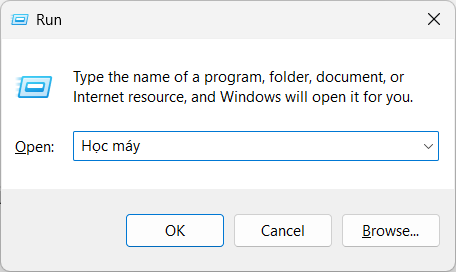
\includegraphics[width=8.84cm]{image1.png}
  \caption{Cửa sổ chạy chương trình RUN}
  \label{fig:run-1}
\end{figure}

\begin{figure}[H]
  \centering
  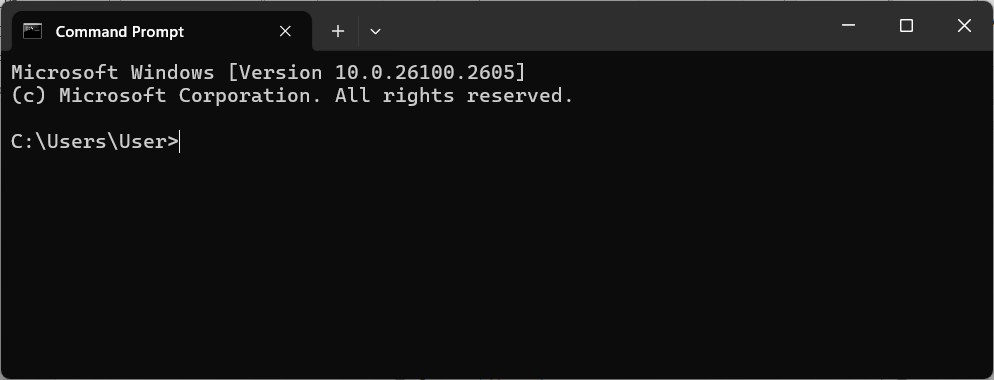
\includegraphics[width=11.12cm]{image2.png}
  \caption{Cửa sổ CMD}
  \label{fig:cmd-1}
\end{figure}

\begin{table}[H]
  \centering
  \caption{Danh sách cán bộ lớp}
  \label{tab:can-bo-lop}
  \begin{tabular}{|C|C|C|}
    \hline
     &  &  \\ \hline
     &  &  \\ \hline
     &  &  \\ \hline
  \end{tabular}
\end{table}

\begin{table}[H]
  \centering
  \caption{Danh sách sinh viên}
  \label{tab:sinh-vien}
  \begin{tabular}{|C|C|C|}
    \hline
     &  &  \\ \hline
     &  &  \\ \hline
  \end{tabular}
\end{table}

\begin{table}[H]
  \centering
  \caption{Danh sách sinh viên K20}
  \label{tab:k20}
  \begin{tabular}{|C|C|C|}
    \hline
     &  &  \\ \hline
     &  &  \\ \hline
  \end{tabular}
\end{table}

\begin{table}[H]
  \centering
  \caption{Danh sách sinh viên K21}
  \label{tab:k21}
  \begin{tabular}{|C|C|C|}
    \hline
     &  &  \\ \hline
     &  &  \\ \hline
  \end{tabular}
\end{table}

\begin{table}[H]
  \centering
  \caption{Danh sách sinh viên K22}
  \label{tab:k22}
  \begin{tabular}{|C|C|C|}
    \hline
     &  &  \\ \hline
     &  &  \\ \hline
  \end{tabular}
\end{table}

\begin{table}[H]
  \centering
  \caption{Danh sách sinh viên K23}
  \label{tab:k23}
  \begin{tabular}{|C|C|C|}
    \hline
     &  &  \\ \hline
     &  &  \\ \hline
  \end{tabular}
\end{table}

\section{Bài toán dự đoán điểm sinh viên}

Nghiên cứu sử dụng các mô hình học máy (Logistic Regression, KNN,
Decision Tree, Random Forest, SVM, XGBoost, CatBoost) để dự đoán tình
trạng tốt nghiệp đúng hạn của sinh viên ngành Ngân hàng (2010--2020).
Kết quả cho thấy Random Forest là mô hình tối ưu, với các thuộc tính như
thông tin học vụ và điểm trung bình học kỳ 1--4 ảnh hưởng mạnh đến khả
năng tốt nghiệp. Nghiên cứu đề xuất giải pháp giúp nâng cao tỷ lệ tốt
nghiệp của sinh viên \cite{hai2017,thuan2022,thuy2023}.

Nghiên cứu áp dụng học máy để dự đoán điểm thi cuối kỳ, tập trung xử lý
dữ liệu mất cân bằng. Phương pháp đạt hiệu suất cao nhất với Precision
43,70\%, Recall 45,1\% và F1-score 44,04\% \cite{lananh,hai2017,thuan2022,thuy2023}.

Theo công trình của Nguyễn Tuấn Anh \cite{alquraishi2021,tuananh2024}

\section{Một số bài toán điển hình}

\subsection{Mục 1}

\subsection{Mục 2}

\subsection{Mục 3}

\section{Kết luận}

% =====================================================================
%  CHƯƠNG 2
% =====================================================================
\chapter{Một số kỹ thuật phân cụm}

\section{Giới thiệu}

\begin{figure}[H]
  \centering
  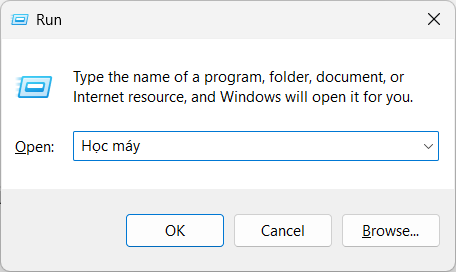
\includegraphics[width=8.84cm]{image1.png}
  \caption{Cửa sổ chạy chương trình RUN}
  \label{fig:run-2}
\end{figure}

\begin{figure}[H]
  \centering
  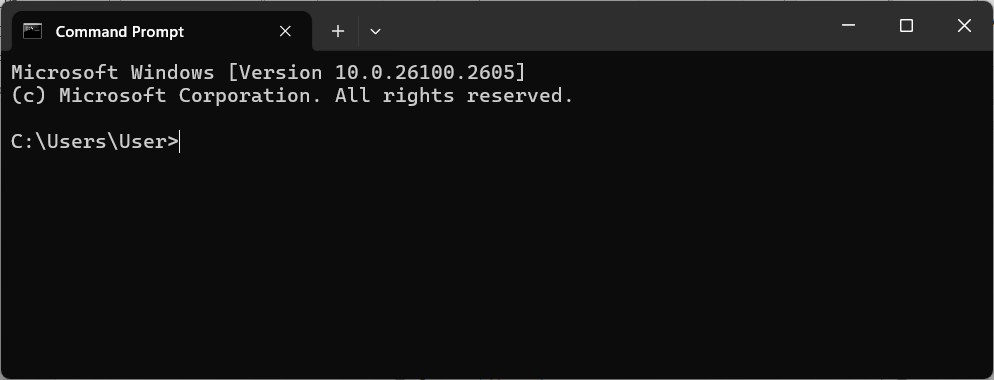
\includegraphics[width=11.12cm]{image2.png}
  \caption{Cửa sổ CMD}
  \label{fig:cmd-2}
\end{figure}

\section{Một số bài toán điển hình}

\subsection{Mục 1}

\subsection{Mục 2}

\subsection{Mục 3}

\section{Kết luận}

% =====================================================================
%  CHƯƠNG 3
% =====================================================================
\chapter{Thử nghiệm và đánh giá}

\section{Giới thiệu}

\begin{figure}[H]
  \centering
  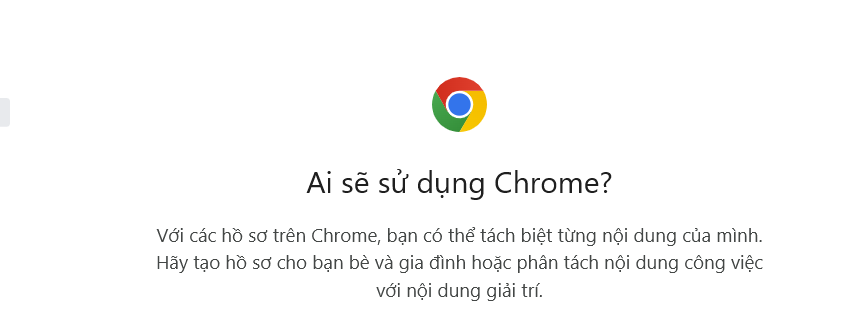
\includegraphics[width=\textwidth]{image3.png}
  \caption{Giao diện Chrome}
  \label{fig:chrome}
\end{figure}

\section{Một số bài toán điển hình}

\subsection{Mục 1}

\subsection{Mục 2}

\subsection{Mục 3}

\section{Phân tích và đánh giá}

\section{Kết luận}

% =====================================================================
%  TÀI LIỆU THAM KHẢO
% =====================================================================
\clearpage
\phantomsection
\addcontentsline{toc}{chapter}{TÀI LIỆU THAM KHẢO}
\begin{thebibliography}{9}

\bibitem{alquraishi2021}
Mohammed AlQuraishi (2021), ``Machine learning in protein structure
prediction'', \textit{Current opinion in chemical biology}. Tập 65, trang: 1--8.

\bibitem{lananh}
Nguyễn Thị Lan Anh, ``Cải thiện kết quả dự đoán điểm thi của sinh viên
bằng Máy học với sự hỗ trợ của R''.

\bibitem{tuananh2024}
Nguyễn Tuấn Anh (2024), ``Ứng dụng mô hình học máy vào trong dự đoán kết
quả học tập của sinh viên tại ICTU'', \textit{Tạp chí Khoa học và Công nghệ ĐHTN}.

\bibitem{hai2017}
Trương Thị Hải, Nguyễn Thái Nghe và Huỳnh Xuân Hiệp (2017), ``Giải pháp
hỗ trợ sinh viên lập kế hoạch học tập dựa trên tiếp cận tập thô'',
\textit{PROCEEDING of Publishing House for Science Technology}.

\bibitem{thuan2022}
Trần Bá Thuấn (2022), ``Ứng dụng machine learning dự báo sinh viên diện
cảnh báo học tập tại trường đại học kinh tế huế'', \textit{Tạp chí Khoa
học Quản lý và Kinh tế, Trường Đại học Kinh Tế, Đại học Huế}. (21).

\bibitem{thuy2023}
Nguyễn Văn Thủy (2023), ``Sử dụng các mô hình Machine Learning dự đoán
tình trạng sinh viên tốt nghiệp đúng hạn'', \textit{Tạp chí Khoa học Đào
tạo Ngân hàng}. Tập 225(8), trang: 52--64.

\end{thebibliography}

\end{document}
